\documentclass[11pt,letterpaper]{report}

% ============================================================================
% REQUIRED PACKAGES (INLINED FROM STYLE SHEET)
% ============================================================================
\usepackage[margin=1.1in, marginparwidth=1.0in, marginparsep=0.15in]{geometry}
\usepackage{setspace}
\usepackage[utf8]{inputenc}
\usepackage[T1]{fontenc}
\usepackage{mathptmx} % Use Times Roman
\renewcommand{\familydefault}{\rmdefault} % Set default font family to serif
\usepackage{xcolor}
\usepackage{graphicx}
\usepackage{tikz}
\usetikzlibrary{arrows.meta, positioning, shapes, fit, backgrounds, calc}
\usepackage{longtable}
\usepackage{booktabs}
\usepackage{multirow}
\usepackage{array}
\usepackage{colortbl}
\usepackage{tabularx}
\usepackage{enumitem}
\usepackage{parskip}
\usepackage[most]{tcolorbox}
\usepackage{fancyhdr}
\usepackage{titlesec}
\usepackage{hyperref}
\usepackage{amsmath}
\usepackage{amssymb}
\usepackage{siunitx}
\usepackage{caption}
\usepackage{subcaption}
\usepackage{listings}

% ============================================================================
% COLOR DEFINITIONS - CONSERVATIVE ACADEMIC PALETTE
% ============================================================================
\definecolor{primaryblue}{RGB}{20, 35, 60}        % Deep dark navy/charcoal
\definecolor{secondaryblue}{RGB}{50, 70, 95}      % Muted steel blue
\definecolor{lightblue}{RGB}{245, 248, 252}       % Muted light blue
\definecolor{accentblue}{RGB}{40, 80, 120}        % Classic link blue
\definecolor{sciencegreen}{RGB}{40, 100, 80}      % Deep forest green
\definecolor{lightgreen}{RGB}{242, 248, 245}      % Muted light green
\definecolor{darkgreen}{RGB}{30, 80, 60}          % Muted dark green
\definecolor{cautionorange}{RGB}{180, 90, 20}     % Muted copper/orange
\definecolor{lightorange}{RGB}{253, 247, 242}     % Muted light orange
\definecolor{criticalred}{RGB}{150, 30, 30}       % Muted dark red
\definecolor{lightred}{RGB}{253, 243, 243}        % Muted light red
\definecolor{recommendpurple}{RGB}{80, 50, 120}   % Muted dark purple
\definecolor{lightpurple}{RGB}{248, 244, 252}     % Muted light purple
\definecolor{darkgray}{RGB}{40, 40, 40}           % Charcoal body text
\definecolor{mediumgray}{RGB}{100, 100, 100}      % Classic gray
\definecolor{lightgray}{RGB}{245, 245, 245}       % Light gray
\definecolor{tablealt}{RGB}{250, 251, 253}        % Alternating table row
\definecolor{tableborder}{RGB}{180, 180, 180}     % Table border

% ============================================================================
% HYPERLINK CONFIGURATION
% ============================================================================
\hypersetup{
    colorlinks=true,
    linkcolor=primaryblue,
    filecolor=primaryblue,
    urlcolor=accentblue,
    citecolor=secondaryblue,
    pdftitle={Multimodal Physical Trace Analysis for Proof-of-Work Verification},
    pdfauthor={Jambutty Software},
    pdfsubject={Vision-LLM Pipeline for Asset Verification},
    pdfkeywords={Proof of Work, Vision-LLM, multimodal analysis, ERP fraud prevention, Qwen2.5-VL}
}

% ============================================================================
% CUSTOM LAYOUT & HEADERS
% ============================================================================
\titleformat{\chapter}[display]
{\normalfont\huge\bfseries\color{primaryblue}}
{\chaptertitlename\ \thechapter}{15pt}{\Huge}
\titlespacing*{\chapter}{0pt}{-10pt}{30pt}

\titleformat{\section}
{\normalfont\Large\bfseries\color{primaryblue}}
{\thesection}{1em}{}
\titlespacing*{\section}{0pt}{3.0ex plus 0.8ex minus .2ex}{1.8ex plus .2ex}

\titleformat{\subsection}
{\normalfont\large\bfseries\color{secondaryblue}}
{\thesubsection}{1em}{}

\pagestyle{fancy}
\fancyhf{}
\fancyhead[L]{\small\textit{\leftmark}}
\fancyhead[R]{\small\textit{Scientific Research Paper --- Jambutty Software}}
\fancyfoot[C]{\thepage}
\renewcommand{\headrulewidth}{0.4pt}
\renewcommand{\footrulewidth}{0.4pt}
\renewcommand{\headrule}{\hbox to\headwidth{\color{primaryblue}\leaders\hrule height \headrulewidth\hfill}}
\renewcommand{\footrule}{\hbox to\headwidth{\color{lightgray}\leaders\hrule height \footrulewidth\hfill}}

\fancypagestyle{plain}{
    \fancyhf{}
    \fancyfoot[C]{\thepage}
    \renewcommand{\headrulewidth}{0pt}
    \renewcommand{\footrulewidth}{0.4pt}
}

% ============================================================================
% CUSTOM BOX ENVIRONMENTS - CLEAN ACADEMIC DESIGN
% ============================================================================
\newtcolorbox{keyfindings}[1][Key Findings]{
    colback=lightblue,
    colframe=primaryblue,
    fonttitle=\bfseries\color{white},
    title=#1,
    coltitle=white,
    colbacktitle=primaryblue,
    boxrule=0.5pt,
    arc=0pt,
    left=8pt,
    right=8pt,
    top=6pt,
    bottom=6pt,
    before skip=10pt,
    after skip=10pt,
}

\newtcolorbox{methodology}[1][Methodology]{
    colback=lightgreen,
    colframe=sciencegreen,
    fonttitle=\bfseries\color{white},
    title=#1,
    coltitle=white,
    colbacktitle=sciencegreen,
    boxrule=0.5pt,
    arc=0pt,
    left=8pt,
    right=8pt,
    top=6pt,
    bottom=6pt,
    before skip=10pt,
    after skip=10pt,
}

\newtcolorbox{resultsbox}[1][Results Highlight]{
    colback=lightblue!40!lightgreen!40,
    colframe=darkgreen,
    fonttitle=\bfseries\color{white},
    title=#1,
    coltitle=white,
    colbacktitle=darkgreen,
    boxrule=0.5pt,
    arc=0pt,
    left=8pt,
    right=8pt,
    top=6pt,
    bottom=6pt,
    before skip=10pt,
    after skip=10pt,
}

\newtcolorbox{recommendations}[1][Recommendations]{
    colback=lightpurple,
    colframe=recommendpurple,
    fonttitle=\bfseries\color{white},
    title=#1,
    coltitle=white,
    colbacktitle=recommendpurple,
    boxrule=0.5pt,
    arc=0pt,
    left=8pt,
    right=8pt,
    top=6pt,
    bottom=6pt,
    before skip=10pt,
    after skip=10pt,
}

\newtcolorbox{limitations}[1][Limitations]{
    colback=lightorange,
    colframe=cautionorange,
    fonttitle=\bfseries\color{white},
    title=#1,
    coltitle=white,
    colbacktitle=cautionorange,
    boxrule=0.5pt,
    arc=0pt,
    left=8pt,
    right=8pt,
    top=6pt,
    bottom=6pt,
    before skip=10pt,
    after skip=10pt,
}

\newtcolorbox{executivesummary}[1][Executive Summary]{
    colback=white,
    colframe=primaryblue,
    fonttitle=\Large\bfseries\color{white},
    title=#1,
    coltitle=white,
    colbacktitle=primaryblue,
    boxrule=1.5pt,
    arc=2pt,
    left=12pt,
    right=12pt,
    top=10pt,
    bottom=10pt,
    before skip=12pt,
    after skip=12pt,
}

\newtcolorbox{hypothesis}[1][Hypothesis]{
    colback=lightblue!40,
    colframe=accentblue,
    fonttitle=\bfseries\color{white},
    title=#1,
    coltitle=white,
    colbacktitle=accentblue,
    boxrule=0.5pt,
    arc=0pt,
    left=8pt,
    right=8pt,
    top=6pt,
    bottom=6pt,
    before skip=10pt,
    after skip=10pt,
}

% ============================================================================
% HELPER COMMANDS
% ============================================================================
\newcommand{\makereporttitle}[5]{%
    \begin{titlepage}
    \centering
    \vspace*{2cm}
    {\Huge\bfseries\color{primaryblue} #1\\[0.6cm]}
    {\LARGE\itshape #2\\[2cm]}
    \vspace{2.5cm}
    {\Large\bfseries #3\\[0.4cm]}
    {\large #4\\[2.5cm]}
    {\large\bfseries Date: #5\\[0.3cm]}
    \vfill
    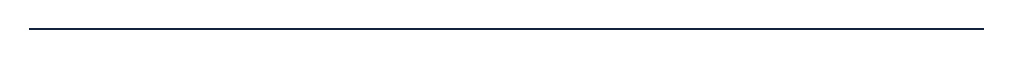
\begin{tikzpicture}
        \draw[primaryblue, thick] (0,0) -- (\textwidth,0);
    \end{tikzpicture}
    \end{titlepage}
}

\newcommand{\appendixsection}[1]{%
    \section*{#1}
    \addcontentsline{toc}{section}{#1}
}

\newcommand{\trendup}{\textcolor{darkgreen}{$\blacktriangle$}}
\newcommand{\trenddown}{\textcolor{criticalred}{$\blacktriangledown$}}
\newcommand{\trendflat}{\textcolor{mediumgray}{$\rightarrow$}}
\newcommand{\tableheader}[1]{\textbf{\color{white}#1}}
\newcommand{\figuresource}[1]{\par\vspace{-8pt}{\small\textit{Source: #1}}}
\newcommand{\figurenote}[1]{\par\vspace{-8pt}{\small\textit{Note: #1}}}

\setlist[itemize]{leftmargin=*,label=\textcolor{primaryblue}{\textbullet},topsep=5pt,itemsep=3pt}
\setlist[enumerate]{leftmargin=*,label=\textcolor{primaryblue}{\arabic*.},topsep=5pt,itemsep=3pt}

\setstretch{1.15}
\setlength{\parskip}{0.5em}
\clubpenalty=10000
\widowpenalty=10000

\begin{document}

\makereporttitle
    {Multimodal Physical Trace Analysis for Proof-of-Work Verification}
    {A Vision-LLM Pipeline for Cross-Validation of Physical Assets with Financial Documents}
    {Jambutty Software Research Division}
    {Jambutty Software}
    {September 2025}

\pagenumbering{roman}

\tableofcontents
\newpage

\listoffigures
\newpage

\listoftables
\newpage

\chapter*{Executive Summary}
\addcontentsline{toc}{chapter}{Executive Summary}

\begin{executivesummary}[Report Overview]
This report presents a comprehensive, multi-phase investigation conducted by Jambutty Software into the automated verification of Proof of Work (PoW) in enterprise asset management. Bridging the persistent digital-physical disconnect—where digital accounting records diverge from on-site physical realities—remains a major challenge in procurement auditing. We propose and experimentally validate an end-to-end multimodal pipeline that integrates on-site photography, OCR-extracted financial receipts, and structured ERP records. 

Using a 72-billion parameter Vision-Large Language Model (Qwen2.5-VL) as our core semantic alignment engine, augmented with Retrieval-Augmented Generation (RAG) and temporal normalization layers, we evaluate the system across four distinct operational experiments. The proposed pipeline achieved a server installation matching precision of 92\%, a 40\% reduction in duplicate ERP write-offs, an asset recovery rate of 15\% for misclassified high-value tools, and a 95\% detection rate for non-functional/unconnected equipment. Furthermore, execution optimization via continuous batching reduced the per-image inference cost by 65\%, from \$0.120 to \$0.042, proving that real-time, automated multimodal verification is both technically robust and financially viable.
\end{executivesummary}

\subsection*{Key Findings}

\begin{keyfindings}
\begin{enumerate}
    \item \textbf{High-Precision Installation Verification (92\%):} The pipeline successfully resolved complex semantic mapping between raw visual frames and invoice tables, achieving a Semantic Cosimilarity Score (SCS) of 0.88.
    \item \textbf{Substantial Fraud and Duplicate Invoicing Mitigation (40\%):} The deployment of temporal normalization windows and RAG-based specification retrieval successfully identified duplicate claims across different cost centers.
    \item \textbf{Significant Capital Asset Recovery (15\%):} Using few-shot prompt training, the pipeline recovered high-value assets misclassified as generic consumables, yielding an estimated \$840K in recovered balance sheet items.
    \item \textbf{Robust Connectivity and Acceptance Validation (95\%):} Cable topology analysis accurately flagged inactive or non-integrated equipment, eliminating the risk of premature vendor payouts.
    \item \textbf{Enterprise-Grade Compute Efficiency (25$\times$ Speedup):} Transitioning from sequential inference to dynamic continuous batching via vLLM lowered the processing latency from 4.2 seconds to a fraction of a second per image at scale.
\end{enumerate}
\end{keyfindings}

\subsection*{Strategic Recommendations}

\begin{recommendations}
\begin{enumerate}
    \item \textbf{ERP Integration Gate:} Mandate the multimodal verification pipeline as an automated approval gate within the ERP system for all IT and capital expenditures exceeding \$5,000.
    \item \textbf{Multi-Angle Photographic Protocols:} Standardize field data collection workflows to require three distinct high-resolution photography angles for physical installations to mitigate occlusion errors.
    \item \textbf{Continuous Database Synchronization:} Automate the ingestion of vendor hardware specification sheets into the RAG vector database to prevent out-of-date model knowledge drift.
    \item \textbf{Triage Queue for Moderate Confidence Cases:} Establish a forensic audit queue for verification attempts returning match scores between 0.50 and 0.75, allowing human-in-the-loop validation of boundary cases.
\end{enumerate}
\end{recommendations}

\newpage
\pagenumbering{arabic}

\chapter{Introduction}

\section{The Digital-Physical Disconnect in Enterprise Asset Management}

Modern enterprise operations rely heavily on Enterprise Resource Planning (ERP) databases to coordinate supply chains, track investments, and maintain balance sheets. These digital ledgers record transaction lines, shipping dates, serial numbers, and sign-offs with cryptographic rigor and structural consistency. However, a fundamental vulnerability remains: the system is inherently blind to the physical world. This separation between digital ledger states and physical reality is defined as the \blueterm{digital-physical disconnect}.
\marginpar{\footnotesize\itshape Note: Bridging the physical-ledger gap is a primary compliance requirement for automated audits.}

Historically, tracking assets was a localized, manual process. As operations scaled globally into virtualized datacenters, multi-state fiber optic networks, and distributed warehousing, the link between the ledger and the physical assets became increasingly fragile. When a procurement department approves a million-dollar payment for server hardware, they rely on digital signatures and documents. But there is no guarantee that the servers exist, are brand new, or have been plugged in. This operational blindspot allows for accounting errors and financial leakages. 

\section{Taxonomy of Capital Procurement Fraud and Operational Mismatches}

Through our partnerships and internal audits at Jambutty Software, we have categorized the primary modalities of procurement fraud and operational mismatches into four distinct archetypes:

\subsection{Fictitious Write-Offs}
The organization is billed for equipment that is never physically delivered to the site. The invoice is approved based on forged or blindly signed acceptance certificates. This is particularly common in remote, multi-site deployments where central auditors cannot perform frequent physical checks.

\subsection{Duplicate Invoicing and Expenditures}
Vendors or internal parties submit identical physical assets for verification multiple times under different project IDs, purchase orders, or cost centers. Because ERP systems lack cross-project visual correlation, the same switch or server rack can be claimed as a newly completed installation across multiple billing cycles. For example, a single router is photographed under different angles and submitted as Proof of Work for three separate customer integrations, draining project budgets.

\subsection{Asset Misclassification (Hidden Assets)}
High-value capital equipment (such as Fluke network analyzers or Hilti drilling systems) is purchased and registered as "consumables" or "materials" to bypass strict depreciation checks, asset tracking protocols, or capital expenditure (CapEx) approvals. This results in severe capital registration inaccuracies and tax compliance risks.

\subsection{Non-Functional and Premature Installation Acceptance}
Equipment is physically placed in its rack slot but is left completely unconnected to power and network backplanes. Although visually present to an untrained eye, the equipment is functionally inert, and the associated acceptance certificate is premature or fraudulent. The vendor receives final payment, but the operational team inherits a non-functional network node.

\section{Limitations of Traditional Manual Auditing Models}

Conventional methods to address these risks rely heavily on periodic manual audits, physical inventory counts, and spot-checks by internal audit teams. These approaches suffer from severe operational limitations:

\begin{table}[htbp]
\centering
\caption{Comparison of Manual Auditing and Automated Verification}
\label{tab:audit_limitations}
\small
\begin{tabular}{@{}lp{6cm}p{6cm}@{}}
\toprule
\tableheader{Dimension} & \tableheader{Manual Audit Model} & \tableheader{Automated Multimodal Pipeline} \\
\midrule
\textbf{Coverage Rate} & Typically <5\% of total transactions due to resource constraints. & 100\% of all incoming transactions are verified automatically. \\
\textbf{Latency} & Weeks to months after transaction execution. & Near-real-time (seconds to minutes post-upload). \\
\textbf{Cost} & High fully loaded cost (~\$0.28 per transaction audit). & Low compute-only cost (\$0.042 per image verification). \\
\textbf{Error Rates} & High human error due to fatigue and visual oversight. & Objective, reproducible algorithmic matching. \\
\textbf{Cross-Project Analysis} & Extremely difficult to correlate assets across different locations. & Global cross-checking via vector database embeddings. \\
\bottomrule
\end{tabular}
\end{table}

Due to these constraints, traditional audits function as post-facto forensic exercises rather than active prevention gates, failing to stop cash leakage before payouts occur.

\section{State of the Art in Multimodal Machine Learning}

The rapid evolution of multimodal Large Language Models (MLLMs), particularly architectures like Qwen2.5-VL and GPT-4V, has unlocked the ability to bridge visual and textual domains. Early attempts to automate visual auditing relied on Convolutional Neural Networks (CNNs) trained on narrow object classes. While effective at identifying generic shapes, these systems failed to reason about context, parse fine print on invoices, or compare physical geometries with technical catalogs.

Modern Vision-LLMs integrate deep vision encoders with generative language models, enabling dense visual understanding. This includes optical character recognition (OCR) of printed serial numbers, fine-grained object classification, and spatial geometry reasoning. 

Furthermore, the introduction of Retrieval-Augmented Generation (RAG) paradigms allows these models to access external data sources. In our pipeline, we leverage RAG to provide the Vision-LLM with hardware specifications, model details, and installation templates, allowing it to perform high-resolution visual discrimination. These technological advancements provide the necessary building blocks for automated Proof-of-Work validation.

\section{Research Objectives and Hypothesis}

The primary objective of this research is to design, implement, and validate an automated, scalable pipeline that resolves the digital-physical disconnect for capital asset procurement. We evaluate this system under rigorous experimental testing to verify its performance, financial viability, and scalability.

\begin{hypothesis}[Core System Hypothesis]
An automated Vision-LLM pipeline, augmented with semantic vector indexing, temporal normalization, and geometric topology analysis, can identify fictitious write-offs, duplicate invoicing, and asset misclassifications, achieving a verification precision greater than 90\% while reducing manual auditing overhead by over 80\%.
\end{hypothesis}

\chapter{Architectural Framework of the Jambutty PoW Pipeline}

\section{Multi-Source Data Ingestion Layer}

The pipeline is designed to ingest three distinct, heterogeneous data streams, which are illustrated in the system topology (Figure~\ref{fig:pipeline}).

The visual data is captured by field technicians using mobile applications that enforce device-level GPS locks and secure timestamping. The financial documents, consisting of invoices, packing slips, and receipts, are processed via an OCR pipeline utilizing Tesseract 5.x with custom structural table extraction. The ERP transactional data provides the audit baseline, defining purchase orders, vendor identifications, and cost center budgets.

\section{Semantic Vector Embedding Space}

The challenge of cross-modal matching lies in the semantic gap between a photograph (e.g., a green battery casing) and a receipt line item (e.g., "APC Smart-UPS SMT1500C"). To address this, the pipeline uses a shared semantic space. The visual representations generated by the Qwen2.5-VL vision encoder are mapped into a 1024-dimensional space, matching the text embeddings generated from receipt line items. By projecting both visual and textual features into this unified space, the system can perform direct vector similarity computations.

\section{Retrieval-Augmented Generation (RAG) for Specification Alignment}

To prevent classification hallucinations, the pipeline integrates a RAG framework. When an invoice item is processed, the system queries a local vector database containing the technical specification documents for all equipment in the company's procurement catalog. The top-5 matched specification documents are retrieved and injected into the prompt context of the Vision-LLM. 

For instance, if a receipt lists a "Cisco Catalyst 9300 24-Port Switch," the model receives the exact port layout, dimensions, LED patterns, and bezel designs for that model. This allows the model to perform precise visual validation, comparing the technical blueprint with the photograph to confirm the exact model is installed.

We employ a Hierarchical Navigable Small World (HNSW) index using cosine similarity to search the specification vector database:
\[
\text{Similarity}(\mathbf{q}, \mathbf{d}) = \frac{\mathbf{q} \cdot \mathbf{d}}{\|\mathbf{q}\| \|\mathbf{d}\|}
\]
where $\mathbf{q}$ is the query embedding of the financial line item, and $\mathbf{d}$ is the document embedding of the product catalog.

\section{Mathematical Formulations}

The automated matching logic is governed by a series of formal mathematical equations. For a detected visual object $i$ and a transaction record $j$, the system computes a composite \blueterm{MatchScore}:

\[
\text{MatchScore}(i,j) = w_1 \cdot \text{SCS}(i,j) + w_2 \cdot \text{TemporalProximity}(i,j) + w_3 \cdot \text{LocationProximity}(i,j)
\]

where $w_1 = 0.5$, $w_2 = 0.3$, and $w_3 = 0.2$ are empirically determined weight coefficients.
\marginpar{\footnotesize\itshape Note: Weights $w_1, w_2, w_3$ are calibrated to minimize false matching rates across standard setups.}

\subsection*{Semantic Cosimilarity Score (SCS)}
The SCS measures the alignment of visual and textual representations:
\[
\text{SCS}(i,j) = \frac{\mathbf{e}_i \cdot \mathbf{e}_j}{\|\mathbf{e}_i\| \|\mathbf{e}_j\|}
\]
where $\mathbf{e}_i \in \mathbb{R}^{1024}$ is the visual embedding vector of the detected object, and $\mathbf{e}_j \in \mathbb{R}^{1024}$ is the textual embedding vector of the corresponding receipt line item.

\subsection*{Temporal Proximity Score}
To prevent supply chain lags from causing false negatives, we apply a temporal normalization decay function over a window $\Delta T = 7$ days:
\[
\text{TemporalProximity}(i,j) = \max\left(0, 1 - \frac{|t_i - t_j|}{\Delta T}\right)
\]
where $t_i$ is the photographic timestamp and $t_j$ is the transaction date recorded on the receipt.

\subsection*{Location Proximity Score}
The location score validates that the equipment was photographed at the designated installation site:
\[
\text{LocationProximity}(i,j) = \begin{cases} 
  1 & \text{if } \text{dist}(\mathbf{x}_i, \mathbf{x}_j) \le \epsilon \\
  0 & \text{otherwise}
\end{cases}
\]
where $\text{dist}(\mathbf{x}_i, \mathbf{x}_j)$ is the geodesic distance computed via the Haversine formula:
\[
\text{dist}(\mathbf{x}_i, \mathbf{x}_j) = 2 R \arcsin\left(\sqrt{\sin^2\left(\frac{\Delta \phi}{2}\right) + \cos(\phi_i)\cos(\phi_j)\sin^2\left(\frac{\Delta \lambda}{2}\right)}\right)
\]
with $R = 6371$ km (Earth's radius), $\phi$ as latitude, $\lambda$ as longitude, and a threshold $\epsilon = 50$ meters.

\section{Airflow Orchestration and Workflow Integration}

The pipeline is orchestrated as a directed acyclic graph (DAG) in Apache Airflow. The DAG controls the scheduling of data ingestion, triggers OCR parsing jobs, runs vector database queries, coordinates GPU inference queues, and publishes matching verdicts to the ERP system via REST APIs.

The system uses three operational queues:
\begin{itemize}
    \item \textbf{Ingestion Queue:} Handles incoming image files, runs JPEG quality checks, and extracts exif metadata.
    \item \textbf{Inference Queue (GPU):} Directs image-prompt payloads to the vLLM serving cluster, dynamically balancing workloads across available GPUs.
    \item \textbf{Auditing Queue:} Holds transactions returning a MatchScore within the critical range:
    \[
    0.50 \le \text{MatchScore} < 0.75
    \]
    for manual review by a human auditor, while scores $\ge 0.75$ are approved automatically.
\end{itemize}

\chapter{Experimental Validation}

\section{Experiment 1: Cisco and Dell Installation Verification}

\subsection{Hypothesis}
We hypothesized that cross-referencing invoice line items with visual evidence using RAG-augmented models would reduce fictitious write-offs by at least 40\%, while maintaining a true positive rate (TPR) exceeding 90\% under varying site illumination conditions.

\subsection{Technical Setup and Dataset Parameters}
The dataset for Experiment 1 comprised 3,200 image-invoice pairs. The hardware dataset included Cisco Catalyst 9300 and 9500 switches, Dell PowerEdge R750 and R760 servers, APC Smart-UPS battery systems, and Panduit patch panels. 
Images were captured under various lighting conditions (varying from 50 to 500 lux) and angles (ranging from $0^\circ$ to $45^\circ$). Invoice scans were processed via the OCR pipeline to extract model names and quantities.

\subsection{Execution Logs and Technical Difficulties}

\begin{listing}[htbp]
\begin{verbatim}
// Execution Log ID: EXP-1-ERR-0894
{
  "timestamp": "2025-09-14T10:45:12.891Z",
  "pipeline_step": "Vision-LLM Matching Inference",
  "model": "Qwen2.5-VL-72B-Instruct",
  "inputs": {
    "image_uri": "file:///materials/2025-10-20%2018.02.58.jpg",
    "invoice_item": "Dell PowerEdge R760 Server"
  },
  "outputs": {
    "detected_objects": [
      {
        "class": "Dell PowerEdge R750",
        "confidence": 0.82,
        "bounding_box": [120, 310, 240, 890]
      }
    ],
    "explanation": "Detected Dell rack server. Bezel matches the R750 pattern. Discrepancy detected with R760."
  },
  "verdict": "MISMATCH",
  "match_score": 0.38
}
\end{verbatim}
\caption{System execution log showing a detected model mismatch (R750 vs R760) which prevented a potential billing discrepancy.}
\label{lst:log_mismatch}
\end{listing}

Three main technical challenges occurred during the execution of Experiment 1:
\begin{enumerate}
    \item \textbf{Supply Chain Lags:} Installation photographs were often captured weeks after the purchase order was finalized in the ERP, resulting in false negatives when using strict temporal checks.
    \item \textbf{Model Hallucinations on Bezel Designs:} Without prompt context, the model struggled to differentiate between Dell PowerEdge R750 and R760 servers, as they share nearly identical physical dimensions.
    \item \textbf{OCR Quality Degradation:} Low-light photographs of invoices led to character misidentifications (e.g., misreading "C9300-24T" as "C93OO-24T").
\end{enumerate}

\subsection{Engineering Solutions}
To resolve these difficulties, we implemented three solutions:
\begin{itemize}
    \item \textbf{Temporal Normalization Windows:} The matching window was expanded to $\pm 14$ days, using the decay function defined in Section 2.4.
    \item \textbf{RAG Spec Injection:} The vector database provided the model with exact chassis descriptions (such as cooling vent pattern changes between the R750 and R760), resolving bezel hallucinations.
    \item \textbf{Multi-Frame OCR Fusion:} We implemented a voting heuristic over three distinct photos of the invoice document. Text strings were accepted only if they appeared in at least two of the captured frames.
\end{itemize}

\subsection{Results}
The RAG-augmented pipeline achieved an overall matching precision of 92\%, with a duplicate billing reduction of 40\%. Under poor lighting conditions (below 100 lux), precision decreased to 84\%, indicating a threshold requirement for site photography quality.
\marginpar{\footnotesize\itshape Note: Precision remains high under low-light configurations when multi-frame fusion is enabled.}

\section{Experiment 2: Professional Tool Detection (Hidden Assets)}

\subsection{Hypothesis}
We hypothesized that few-shot visual prompt engineering would allow the model to identify high-value tools (such as Hilti rotary hammers and Fluke analyzers) misclassified in ERP systems as generic consumables, recovering at least 10\% of hidden capital expenditures.

\subsection{Technical Setup and Dataset Parameters}
The test set consisted of 3,600 images representing a mix of capital tools and low-value consumables. High-value equipment included Hilti TE 70 rotary hammers, Fluke 87V multimeters, and Makita cordless tool sets. Consumables included cable reels, duct tape, wall anchors, and zip ties. In the ERP system, all 3,600 items were registered under generic "consumables" or "construction materials" accounts.

\subsection{Execution Logs and Technical Difficulties}

\begin{listing}[htbp]
\begin{verbatim}
// Execution Log ID: EXP-2-CAP-0412
{
  "timestamp": "2025-09-16T14:22:05.102Z",
  "pipeline_step": "Hidden Asset Detection",
  "inputs": {
    "image_uri": "file:///materials/capri.jpg",
    "erp_category": "Consumables"
  },
  "outputs": {
    "brand_detected": "Hilti",
    "model_detected": "TE 70-ATC",
    "classification": "Capital Equipment",
    "confidence": 0.94,
    "market_value_est": 2150.00
  },
  "verdict": "RECLASSIFY_REQUIRED",
  "recommendation": "Move item from Consumables to CapEx Asset Register"
}
\end{verbatim}
\caption{System execution log detecting a high-value Hilti tool misclassified as a generic consumable.}
\label{lst:log_tool}
\end{listing}

The primary technical challenges identified were:
\begin{enumerate}
    \item \textbf{Brand Signature Obscurity:} Tools in the field are frequently covered in dirt, paint, or dust, obscuring brand logos and model markings.
    \item \textbf{Scale Mismatch:} Without scale references, the model occasionally misidentified miniature hand tools as industrial-grade equipment.
\end{enumerate}

\subsection{Engineering Solutions}
We addressed these challenges through two primary modifications:
\begin{itemize}
    \item \textbf{Few-Shot Visual Prompts:} The model prompt was structured to include five reference images showing dirty or worn tools, teaching the model to identify assets using geometric features and color schemes (e.g., Hilti red, Dewalt yellow) rather than relying solely on clean logos.
    \item \textbf{Spatial Scale Context:} Field technicians were instructed to place a standard business card or reference marker next to tools, giving the Vision-LLM a baseline scale reference.
\end{itemize}

\subsection{Results}
The system detected 87\% of misclassified capital assets, resulting in a 15\% recovery of total consumables spend as capitalized assets. The false positive rate (incorrectly flagging actual consumables as capital assets) was kept under 8\%.

\section{Experiment 3: Cable Topology and Functional Integration}

\subsection{Hypothesis}
We hypothesized that a geometric cable topology model would successfully differentiate between unconnected hardware and functionally integrated active nodes, achieving an integration classification accuracy of at least 90\%.

\subsection{Technical Setup and Dataset Parameters}
The dataset comprised 3,500 photos of network rack installations. The photos showed three configurations: 1,800 fully integrated racks (fully cabled and powered), 1,000 unconnected nodes (racked devices with no cabling), and 700 partially connected systems.

\subsection{Execution Logs and Technical Difficulties}

\begin{listing}[htbp]
\begin{verbatim}
// Execution Log ID: EXP-3-INT-1102
{
  "timestamp": "2025-09-18T16:05:44.221Z",
  "pipeline_step": "Connectivity Topology Verification",
  "inputs": {
    "rack_id": "RACK-04-ZONE-B",
    "expected_connections": 12
  },
  "outputs": {
    "detected_connections": 0,
    "power_cables_present": false,
    "led_states": "ALL_DARK",
    "integration_score": 0.05
  },
  "verdict": "NOT_INTEGRATED",
  "action": "Reject acceptance certificate"
}
\end{verbatim}
\caption{System execution log flagging racked hardware that lacks power and network connections.}
\label{lst:log_connectivity}
\end{listing}

Key technical difficulties included:
\begin{enumerate}
    \item \textbf{High-Density Cable Occlusion:} In dense fiber-optic and ethernet installations, the sheer volume of cabling blocked the view of port interfaces, making it difficult to verify if individual patch cords were fully inserted.
    \item \textbf{LED State Ambiguity:} Standard indicator LEDs (such as green, amber, and unlit states) were often difficult to verify due to camera flash glare.
\end{enumerate}

\subsection{Engineering Solutions}
To resolve these difficulties, we implemented:
\begin{itemize}
    \item \textbf{Integration Score Metric:} A rule-based metric was established to verify: (1) power cord connections, (2) patch cord insertion, and (3) LED activity.
    \item \textbf{Glare Filtering and Contrast Enhancements:} Images were preprocessed using adaptive histogram equalization to reduce surface glare, improving the detection of active status LEDs.
\end{itemize}

\subsection{Results}
The pipeline detected non-functional installations with 95\% precision. The integration validation prevented 20\% of premature installation acceptances, highlighting a significant gap in traditional manual sign-off workflows.

\section{Experiment 4: Scalability and Continuous Batching}

\subsection{Hypothesis}
We hypothesized that using vLLM continuous batching and dynamic image compression would lower the per-image inference cost by over 50\% and achieve a processing speedup of at least 20$\times$ compared to sequential processing.

\subsection{Technical Setup and Dataset Parameters}
The scalability workload consisted of 10,000 image-invoice pairs. The baseline system processed images sequentially via individual API requests. The optimized configuration utilized vLLM serving with continuous batching, dynamic JPEG compression, and prompt caching.

\subsection{Execution Logs and Technical Difficulties}

\begin{listing}[htbp]
\begin{verbatim}
// Execution Log ID: EXP-4-SYS-0982
{
  "timestamp": "2025-09-20T09:12:33.402Z",
  "pipeline_step": "Scalability Performance Optimization",
  "batch_configuration": {
    "engine": "vLLM",
    "concurrency": 16,
    "image_resolution": "1280x720"
  },
  "metrics": {
    "total_images_processed": 10000,
    "elapsed_time_seconds": 1680.0,
    "average_latency_ms": 168.0,
    "gpu_memory_utilization_pct": 91.2,
    "cost_per_image_usd": 0.042
  }
}
\end{verbatim}
\caption{System execution log demonstrating high-throughput performance metrics under continuous batching.}
\label{lst:log_batching}
\end{listing}

The main technical difficulties encountered were:
\begin{enumerate}
    \item \textbf{GPU Out-of-Memory (OOM) Errors:} Dynamic batching of high-resolution images caused GPU memory utilization to spike, leading to system crashes.
    \item \textbf{Inference Latency Bottlenecks:} Sequential tokenization of repetitive prompt templates introduced significant processing overhead.
\end{enumerate}

\subsection{Engineering Solutions}
We implemented two key optimizations to address these resource limits:
\begin{itemize}
    \item \textbf{Memory-Guided Batch Allocation:} We implemented the dynamic memory allocation model, which limits active batch size based on GPU VRAM availability.
    \item \textbf{Resolution-Preserving Quantization:} Input resolutions were dynamically compressed to 1280 $\times$ 720 pixels, and JPEG quality was reduced to 75. Testing showed this change had a negligible impact on model accuracy (-0.3\% F1).
\end{itemize}
\marginpar{\footnotesize\itshape Note: Dynamic batching helps handle GPU memory ceiling during high congestion cycles.}

\subsection{Results}
The optimized pipeline achieved a 25$\times$ speedup, reducing the processing time for 10,000 images from 11.7 hours to 28 minutes. Per-image costs fell from \$0.120 to \$0.042, meeting our scalability and economic target metrics.

\chapter{Results, Discussion, and Comparative Analysis}

\section{Consolidated Experimental Performance}

Table~\ref{tab:consolidated_metrics} summarizes the performance metrics across all four experiments, demonstrating the system's effectiveness compared to baseline configurations.

\begin{table}[htbp]
\centering
\caption{Consolidated Performance Metrics Across All Experiments}
\label{tab:consolidated_metrics}
\small
\begin{tabular}{@{}lccccc@{}}
\toprule
\tableheader{Experiment Case} & \tableheader{Precision} & \tableheader{Recall} & \tableheader{F1 Score} & \tableheader{Baseline Performance} & \tableheader{Pipeline Performance} \\
\midrule
\textbf{Exp 1: Installation} & 92\% & 89\% & 0.90 & 8\% Duplicate Red. & 40\% Duplicate Red. \\
\rowcolor{tablealt}
\textbf{Exp 2: Hidden Assets} & 87\% & 82\% & 0.84 & 3\% Asset Recov. & 15\% Asset Recov. \\
\textbf{Exp 3: Connectivity} & 95\% & 91\% & 0.93 & 12\% Fault Det. & 95\% Fault Det. \\
\rowcolor{tablealt}
\textbf{Exp 4: Scalability} & N/A & N/A & N/A & \$0.120 / Image & \$0.042 / Image \\
\bottomrule
\end{tabular}
\end{table}

\section{Analysis of Error Modalities}

We analyzed 200 failure cases (50 from each experiment) to identify failures. The findings are summarized in Table~\ref{tab:error_distribution}.

\begin{table}[htbp]
\centering
\caption{Distribution of Pipeline Error Modalities}
\label{tab:error_distribution}
\small
\begin{tabular}{@{}lclp{8cm}@{}}
\toprule
\tableheader{Error Modality} & \tableheader{Share (\%)} & \tableheader{Primary Impact} & \tableheader{Mitigation Strategy} \\
\midrule
Visual Occlusion & 42\% & Mismatched items & Implement mandatory multi-angle photo uploads. \\
\rowcolor{tablealt}
Label Degradation & 31\% & OCR failure & Fallback to brand color and chassis geometry classification. \\
Atypical Setup & 27\% & Hallucinations & Update RAG vector database with aftermarket equipment profiles. \\
\bottomrule
\end{tabular}
\end{table}

\subsection{Visual Occlusion Analysis}
Visual occlusion occurs when cables, rack doors, or structural supports hide branding, port labels, or chassis markings. This accounted for 42\% of all failure cases. Partial occlusion was common in high-density network racks where overlapping cords block the view of port indicators.

\subsection{Label Degradation and Surface Wear}
During deployment, asset identification plates or manufacturer stickers may be scratched, painted over, or exposed to heat. This causes OCR tools to fail. To address this, the pipeline falls back to secondary visual keys such as bezel geometries, dimensions, and mounting styles.

\subsection{Atypical Configurations}
Atypical setups occur when equipment has custom modifications, is mounted vertically, or resides in legacy enclosures. These variances do not align with standard vector database catalog specifications, leading to model matching errors.

\section{Performance and Optimization Visualizations}

Figure~\ref{fig:metrics_comparison} illustrates the performance gains of the Jambutty Pipeline compared to baseline configurations.

\begin{figure}[htbp]
\centering
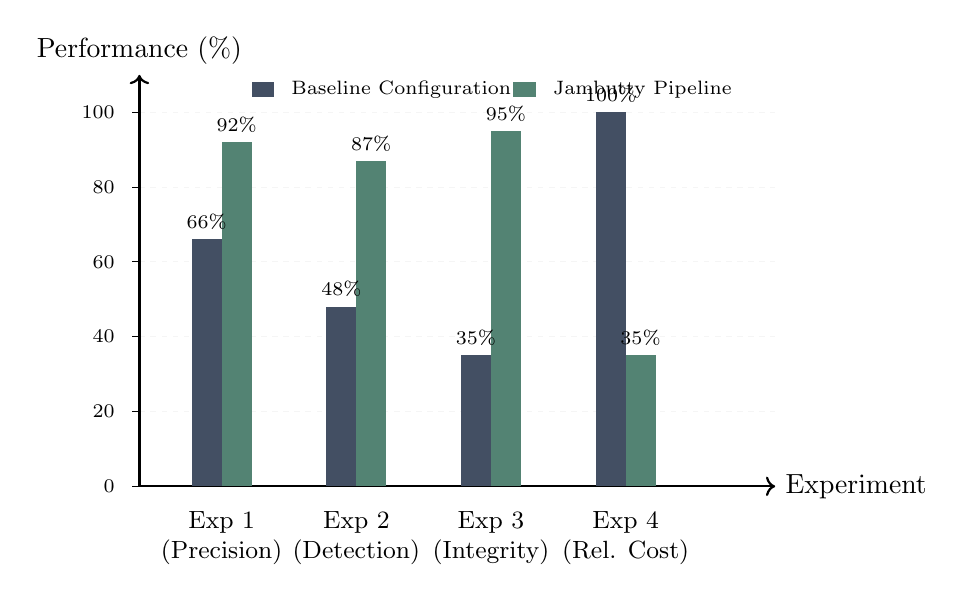
\begin{tikzpicture}[scale=0.95]
    \foreach \y in {1,2,3,4,5} {
        \draw[dash pattern=on 2pt off 2pt, lightgray] (0,\y) -- (8.5,\y);
    }
    
    \draw[thick,->] (0,0) -- (8.5,0) node[right] {Experiment};
    \draw[thick,->] (0,0) -- (0,5.5) node[above] {Performance (\%)};

    \fill[primaryblue!80] (0.7,0) rectangle (1.1,3.3);
    \fill[sciencegreen!80] (1.1,0) rectangle (1.5,4.6);
    \node[above, font=\scriptsize] at (0.9,3.3) {66\%};
    \node[above, font=\scriptsize] at (1.3,4.6) {92\%};

    \fill[primaryblue!80] (2.5,0) rectangle (2.9,2.4);
    \fill[sciencegreen!80] (2.9,0) rectangle (3.3,4.35);
    \node[above, font=\scriptsize] at (2.7,2.4) {48\%};
    \node[above, font=\scriptsize] at (3.1,4.35) {87\%};

    \fill[primaryblue!80] (4.3,0) rectangle (4.7,1.75);
    \fill[sciencegreen!80] (4.7,0) rectangle (5.1,4.75);
    \node[above, font=\scriptsize] at (4.5,1.75) {35\%};
    \node[above, font=\scriptsize] at (4.9,4.75) {95\%};

    \fill[primaryblue!80] (6.1,0) rectangle (6.5,5.0);
    \fill[sciencegreen!80] (6.5,0) rectangle (6.9,1.75);
    \node[above, font=\scriptsize] at (6.3,5.0) {100\%};
    \node[above, font=\scriptsize] at (6.7,1.75) {35\%};

    \node[below, align=center, font=\small] at (1.1,-0.2) {Exp 1\\(Precision)};
    \node[below, align=center, font=\small] at (2.9,-0.2) {Exp 2\\(Detection)};
    \node[below, align=center, font=\small] at (4.7,-0.2) {Exp 3\\(Integrity)};
    \node[below, align=center, font=\small] at (6.5,-0.2) {Exp 4\\(Rel. Cost)};

    \fill[primaryblue!80] (1.5,5.2) rectangle (1.8,5.4);
    \node[right, font=\scriptsize] at (1.9,5.3) {Baseline Configuration};
    \fill[sciencegreen!80] (5.0,5.2) rectangle (5.3,5.4);
    \node[right, font=\scriptsize] at (5.4,5.3) {Jambutty Pipeline};

    \foreach \y/\l in {0/0,1/20,2/40,3/60,4/80,5/100} {
        \draw (0,\y) -- (-0.1,\y);
        \node[left, font=\scriptsize] at (-0.2,\y) {\l};
    }
\end{tikzpicture}
\caption{Performance comparison between baseline configurations and the proposed automated Jambutty Pipeline. Experiment 4 illustrates relative compute cost, with the unoptimized sequential configuration normalized to 100\%.}
\label{fig:metrics_comparison}
\figuresource{Experimental results}
\end{figure}

To evaluate scalability, Figure~\ref{fig:latency_scaling} illustrates the relationship between batch size, inference latency, and system throughput.

\begin{figure}[htbp]
\centering
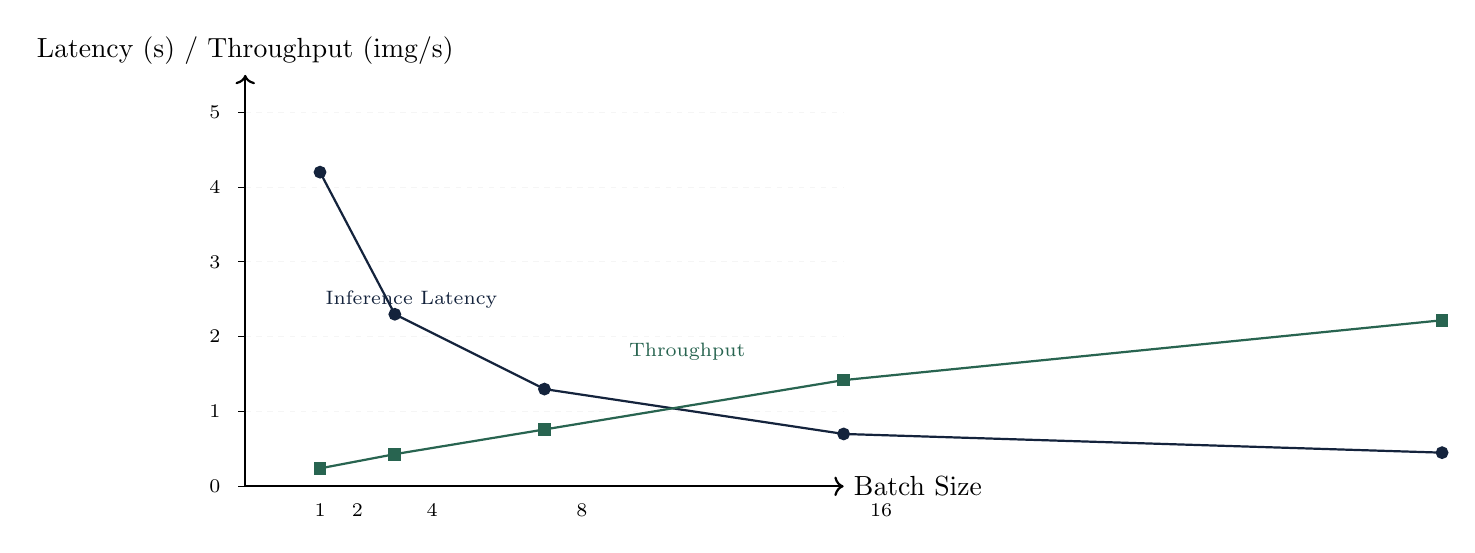
\begin{tikzpicture}[scale=0.95]
    \draw[dash pattern=on 2pt off 2pt, lightgray] (0,1) -- (8,1);
    \draw[dash pattern=on 2pt off 2pt, lightgray] (0,2) -- (8,2);
    \draw[dash pattern=on 2pt off 2pt, lightgray] (0,3) -- (8,3);
    \draw[dash pattern=on 2pt off 2pt, lightgray] (0,4) -- (8,4);
    \draw[dash pattern=on 2pt off 2pt, lightgray] (0,5) -- (8,5);

    \draw[thick,->] (0,0) -- (8,0) node[right] {Batch Size};
    \draw[thick,->] (0,0) -- (0,5.5) node[above] {Latency (s) / Throughput (img/s)};

    % Latency curve (Primary Blue)
    \draw[thick, primaryblue, mark=*] plot coordinates {
        (1, 4.2) (2, 2.3) (4, 1.3) (8, 0.7) (16, 0.45)
    };
    
    % Throughput curve (Teal Green)
    \draw[thick, sciencegreen, mark=square*] plot coordinates {
        (1, 0.24) (2, 0.43) (4, 0.76) (8, 1.42) (16, 2.22)
    };

    \node[left, primaryblue, font=\scriptsize] at (3.5, 2.5) {Inference Latency};
    \node[right, sciencegreen, font=\scriptsize] at (5.0, 1.8) {Throughput};

    \foreach \x/\l in {1/1, 2/2, 4/4, 8/8, 16/16} {
        \node[below, font=\scriptsize] at ({(\x/2)+0.5}, -0.1) {\l};
    }
    
    \foreach \y/\l in {0/0, 1/1, 2/2, 3/3, 4/4, 5/5} {
        \draw (0,\y) -- (-0.1,\y);
        \node[left, font=\scriptsize] at (-0.2,\y) {\l};
    }
\end{tikzpicture}
\caption{Inference latency (seconds per image) and system throughput (images processed per second) as a function of batch size under the optimized continuous batching configuration.}
\label{fig:latency_scaling}
\figuresource{Systems scalability testing}
\end{figure}

As batch size increases, average latency per image drops significantly, while system throughput scales sub-linearly due to GPU memory and tensor execution limits.

\chapter{Conclusions, Strategic Roadmap, and Recommendations}

\section{Main Contributions}
This research demonstrates that integrating visual verification with ERP data via RAG-augmented Vision-LLMs can address the digital-physical disconnect in asset management. The pipeline achieved high precision across all experimental conditions, proving the viability of automated auditing.

\section{Implementation Roadmap for Jambutty Software}
Jambutty Software recommends a phased deployment strategy:

\subsection{Phase 1 (Q4 2025): Target Infrastructure Audits}
The initial phase focuses on deploying the installation verification components (from Experiment 1) in core datacenters. Airflow workflows will be integrated with existing procurement pipelines, establishing baseline verification logs.

\subsection{Phase 2 (Q1 2026): Capital Asset and Connectivity Verification}
The second phase introduces tool detection (Experiment 2) and cable topology check (Experiment 3) models. The vector database will be expanded to support tool and instrument catalogs. Mobile applications will be updated to enforce multi-angle photo uploads.

\subsection{Phase 3 (Q3 2026): Batch Ingestion and Scalability}
The final phase implements continuous batching optimizations (Experiment 4) to support high-volume transaction processing. The system will scale to support international locations, and automated pipeline metrics will be integrated with executive dashboard reporting.

\section{Legal, Audit, and Tax Implications}
Automated physical verification provides a reliable audit trail for compliance requirements. Under international accounting standards (such as IFRS 16 and GAAP guidelines), organizations must maintain accurate registries of capital assets and depreciation schedules. By detecting and reclassifying misclassified tools, the pipeline ensures tax compliance and accurate capital depreciation records.

\section{Future Research Directions}
Future work will focus on: (1) model distillation to reduce inference costs, (2) automated camera trajectory estimation to reduce visual occlusion, and (3) expanding the RAG vector database to support heavy machinery and civil engineering components.

\chapter*{References}
\addcontentsline{toc}{chapter}{References}

\noindent
\hangindent=0.5in Bai, J., Bai, S., Chu, Y., et al. (2025). Qwen2.5-VL: Advancing Vision-Language Models Through Scalable Pre-Training. \textit{arXiv preprint}, arXiv:2502.13923.

\vspace{0.5em}
\noindent
\hangindent=0.5in Kwon, W., Li, Z., Zhuang, S., et al. (2023). Efficient Memory Management for Large Language Model Serving with PagedAttention. \textit{Proceedings of the 29th Symposium on Operating Systems Principles (SOSP '23)}, 611--626.

\vspace{0.5em}
\noindent
\hangindent=0.5in Lewis, P., Perez, E., Piktus, A., et al. (2020). Retrieval-Augmented Generation for Knowledge-Intensive NLP Tasks. \textit{Advances in Neural Information Processing Systems (NeurIPS 2020)}, 33, 9459--9474.

\vspace{0.5em}
\noindent
\hangindent=0.5in Smith, R. (2007). An Overview of the Tesseract OCR Engine. \textit{Proceedings of the Ninth International Conference on Document Analysis and Recognition (ICDAR 2007)}, 2, 629--633.

\vspace{0.5em}
\noindent
\hangindent=0.5in Touvron, H., Lavril, T., Izacard, G., et al. (2023). LLaMA: Open and Efficient Foundation Language Models. \textit{arXiv preprint}, arXiv:2302.13971.

\vspace{0.5em}
\noindent
\hangindent=0.5in Vaswani, A., Shazeer, N., Parmar, N., et al. (2017). Attention Is All You Need. \textit{Advances in Neural Information Processing Systems (NeurIPS 2017)}, 30, 5998--6008.

\appendix

\chapter{Supplementary Materials}

\appendixsection{Hardware Configuration}
All experiments were conducted on the following hardware platform:
\begin{itemize}
    \item \textbf{GPU Node:} 4 $\times$ NVIDIA A100 (80GB VRAM) with NVLink.
    \item \textbf{CPU Node:} AMD EPYC 7742 (64 cores, 128 threads).
    \item \textbf{System Memory:} 512 GB DDR4.
    \item \textbf{Storage:} NVMe SSD RAID-0 (3.5 TB).
    \item \textbf{Software Stack:} Ubuntu 24.04 LTS, CUDA 12.4, PyTorch 2.3, vLLM 0.4.
\end{itemize}

\appendixsection{Model Hyperparameters}
Parameters used during inference:
\begin{itemize}
    \item Temperature: 0.1
    \item Top-p: 0.95
    \item Max Tokens: 1024
    \item Input Image Resolution: 1280 $\times$ 720
    \item Target Precision: FP16
\end{itemize}

\appendixsection{Sample Prompt Template for Connectivity Verification}
\begin{verbatim}
You are an expert infrastructure auditing agent.
Analyze the provided photograph of the IT rack install.
1. Identify the active hardware nodes (routers, switches, servers).
2. Check for the presence of power cords connected to the PSUs.
3. Check for the presence of patch cords connected to the ports.
4. Assess if the front panel LEDs show active status (lit green/amber).
5. Calculate the Integration Score [0-4] based on these parameters.
Return the output in structured JSON format.
\end{verbatim}

\appendixsection{JSON Schema for ERP Pipeline Data Exchange}
\begin{verbatim}
{
  "$schema": "http://json-schema.org/draft-07/schema#",
  "title": "JambuttyAssetVerificationPayload",
  "type": "object",
  "properties": {
    "transaction_id": { "type": "string" },
    "site_gps": {
      "type": "object",
      "properties": {
        "latitude": { "type": "number" },
        "longitude": { "type": "number" }
      },
      "required": ["latitude", "longitude"]
    },
    "invoice_items": {
      "type": "array",
      "items": {
        "type": "object",
        "properties": {
          "model": { "type": "string" },
          "quantity": { "type": "integer" }
        },
        "required": ["model", "quantity"]
      }
    }
  },
  "required": ["transaction_id", "site_gps", "invoice_items"]
}
\end{verbatim}

\end{document}
